\subsection{GPR Results}

\lorena{Using GPR to create a map between the injected and recovered masses and
spins of the O2 dataset allows us to better predict the instrisic parameters of 
a binary system. Fig~\ref{m_chi_comparisons} shows the predictions from the O2 
testing dataset. The gray circles represent the recovered values from the 
best-fit template, the orange circles are the predictions coming from regression, 
and the true values are depicted by the black line. Ideally, all values would lie 
along the line.}


%The difference between the recovered and predicted values is 
%clear especially in cases when the recovered masses are very high.  
%Similarly, in Fig.~\ref{m_chi1_chi2_comparisons} the 
%primary spins are closer to the true value using regression. Regression also
%gets rid of highly negative and positive secondary spins that are far from the
%true values. Although both the recovered and the predicted values have seemingly 
%large errors, the predictions improve the overall error significantly.}

\begin{figure}
    \centering
    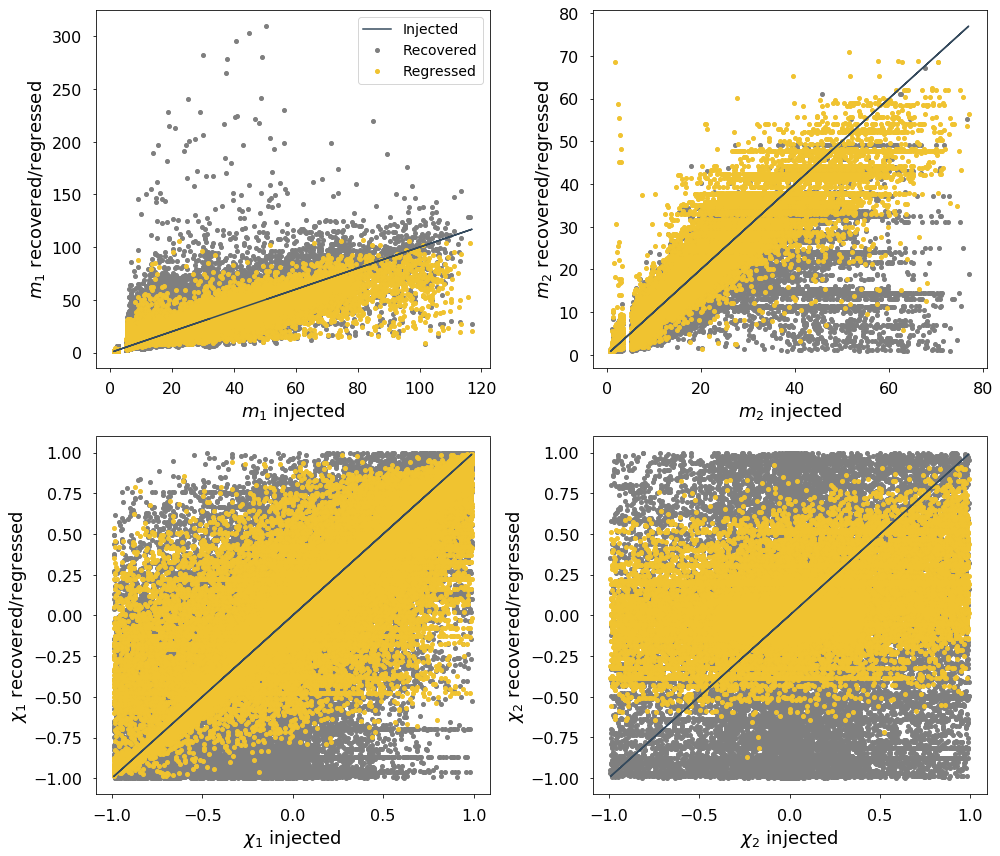
\includegraphics[width=0.45\textwidth]{m_chi_comparisons.png}
    \caption{The top panels show the recovered (gray) and regressed (orange)
             masses as a function of the injected (black line) values. The
             bottom panels show the same functions for the spin magnitudes.
            }
        \label{m_chi_comparisons}
\end{figure}

\lorena{To quantify the above...}
